\documentclass[a4paper]{article} 
\addtolength{\hoffset}{-2.25cm}
\addtolength{\textwidth}{4.5cm}
\addtolength{\voffset}{-3.25cm}
\addtolength{\textheight}{5cm}
\setlength{\parskip}{0pt}
\setlength{\parindent}{0in}

\usepackage[square,sort,comma,numbers]{natbib}
\usepackage{blindtext} % Package to generate dummy text
\usepackage{charter} % Use the Charter font
\usepackage[utf8]{inputenc} % Use UTF-8 encoding
\usepackage{microtype} % Slightly tweak font spacing for aesthetics
\usepackage{amsthm, amsmath, amssymb} % Mathematical typesetting
\usepackage{float} % Improved interface for floating objects
\usepackage{hyperref} % For hyperlinks in the PDF
\usepackage{graphicx, multicol} % Enhanced support for graphics
\usepackage{xcolor} % Driver-independent color extensions
\usepackage{pseudocode} % Environment for specifying algorithms in a natural way
\usepackage[yyyymmdd]{datetime} % Uses YEAR-MONTH-DAY format for dates

\usepackage{fancyhdr} % Headers and footers
\pagestyle{fancy} % All pages have headers and footers
\fancyhead{}\renewcommand{\headrulewidth}{0pt} % Blank out the default header
\fancyfoot[L]{} % Custom footer text
\fancyfoot[C]{} % Custom footer text
\fancyfoot[R]{\thepage} % Custom footer text
\newcommand{\note}[1]{\marginpar{\scriptsize \textcolor{red}{#1}}} % Enables comments in red on margin

%----------------------------------------------------------------------------------------


\newcommand{\yourname}{Schweizerschule Mexiko, CDMX}
\newcommand{\yournetid}{M.Sc. William Bombardelli}
\newcommand{\youremail}{wbombardellis@gmail.com}
\newcommand{\coursename}{Java}

\begin{document}
	\fancyhead[C]{}
\hrule \medskip
\begin{minipage}{0.295\textwidth} 
\raggedright
\footnotesize
\yourname \hfill\\ 
\yournetid \hfill\\ 
\youremail
\end{minipage}
\begin{minipage}{0.3\textwidth} 
\centering 
\large 
Class \assignmentnumber\\ 
\normalsize 
\coursename\\ 
\end{minipage}
\begin{minipage}{0.395\textwidth} 
\raggedleft

\includegraphics[]{logo}\hfill\\
\end{minipage}
\medskip\hrule 
\bigskip

	
	\section{Allgemein}
	\begin{itemize}
		\item Kursname: Java
		\item Lehrer: William Bombardelli
		\item Tempo: 2 Stunden pro Woche. Mittwoch 14.35
	\end{itemize}
	
	\section{Ziele}
	\begin{itemize}
		\item Probleme anhand eines Rechners lösen
		\item Programmen auf Java lesen bzw. verstehen und schreiben 
	\end{itemize}

	\section{Bewertungsprozess}
	\begin{itemize}
		\item 1. Viertel: Mitarbeit
		\item 2. Viertel: 1 Prüfung + 1 benotete Aufgabe
		\item 3. Viertel: 1 Prüfung + 1 benotete Aufgabe
	\end{itemize}

	\section{Bemerkungen}
	\begin{itemize}
		\item Web-Tutorials und Hausaufgaben sind empfohlen aber wahlweise.
		\item Diskussion mit Kollegen und Zusammenarbeit wird gefördert.
		\item Anwesenheit wird jede Woche kontrolliert.
	\end{itemize}

	\section{Literatur und Referenzen}
	\begin{itemize}
		\item Materialien: \url{https://github.com/wbombardellis/java-unterricht}
		\item Oracle Java Tutorial: \url{https://docs.oracle.com/javase/tutorial}
		\item W3C Java Tutorial: \url{https://www.w3schools.com/java}
	\end{itemize}

	\section{Kalender}
	Stand: \the\day/\the\month/\the\year.\\
	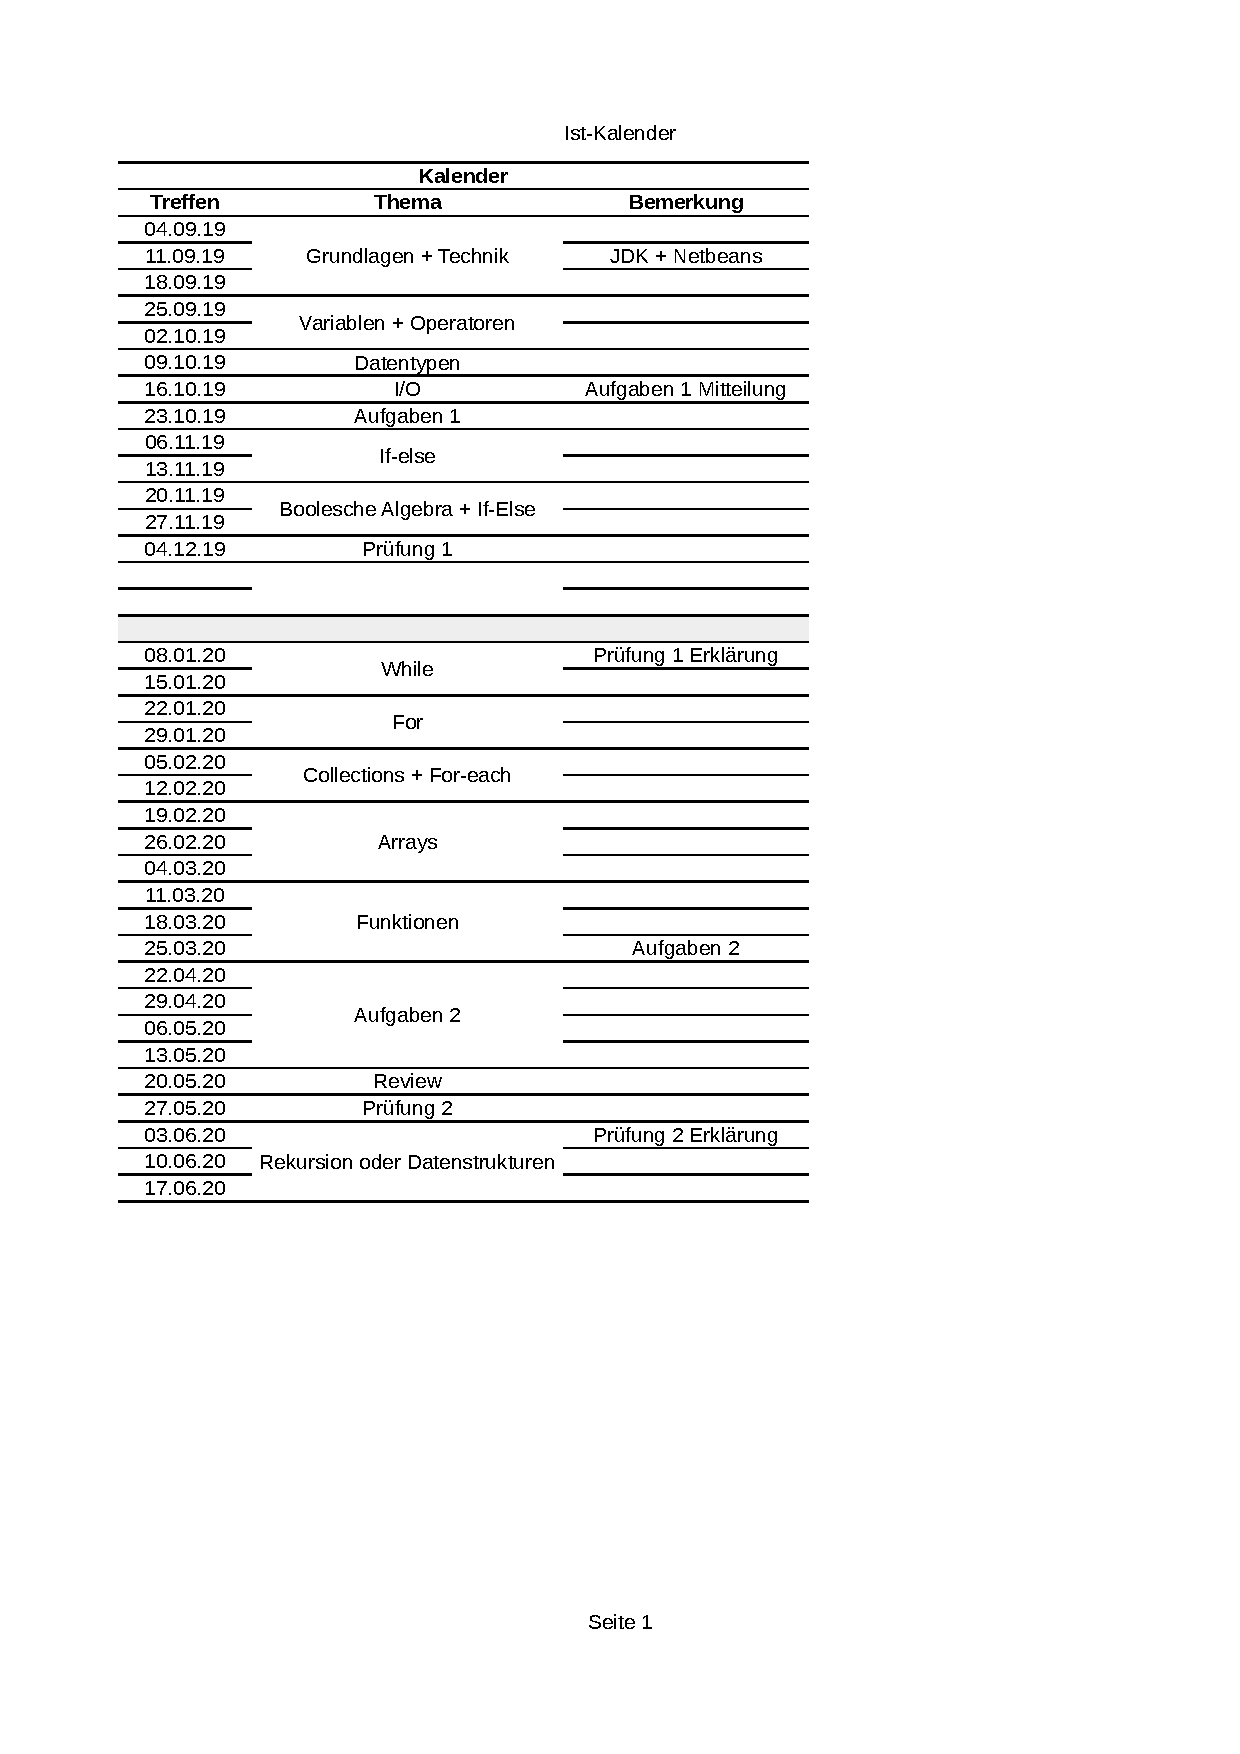
\includegraphics[width=\textwidth]{Kalender}
\end{document}
